\documentclass[11pt,a4paper,twocolumn]{article}
\usepackage{graphicx}
\usepackage{url}
\usepackage[font={it}]{caption}
\usepackage{subcaption}
\usepackage{tikz}

\columnsep +35pt
\graphicspath{./images/}

\usetikzlibrary{trees}

%opening
\title{\textbf{Generating organic game worlds with multi-level spatial partitioning techniques}}
\author{ \small Nico Andrew Glas \\ \small Amsterdam University of Applied Sciences \\ \small Duivendrectsekade 36-38 \\ \small 1096 AH Amsterdam, The Netherlands \\ \small nico.glas@hva.nl}

\begin{document}
\maketitle  

\begin{abstract}
This paper frames the process of generating an organic game world with the use of spatial partitioning techniques. These techniques use sample points to divide a plane into multiple spaces and then using another set of sample points to divide the original spaces. These nested in each other can create even more organic shapes than just one division.
\end{abstract}

\section{Introduction}
When discussing procedural game-content generation, research usually focusses on the generation of missions and levels and such. This in itself is not a real shocker, designing missions and/or levels are one of the most time consuming tasks that game developers face. Many games that use a form of content generation use templates (e.g. Blizzard's \emph{Diablo} series) or, ambiguously named, "Dungeon Generation" as done by \emph{Rogue}. These methods create rather static and monotonous levels as the former could be recognized by keen-minded players, and the latter generating only sterile rectangular shapes that can be seen as rather dull. Another method for content generation is the use of Voronoi diagrams in level and mission generation. This method is a known technique\cite{patel} for the creation of organic game worlds (done by \emph{Realm of the Mad God}), but has its flaws, especially when the details are observed. In this paper I discuss an improved technique using multiple Voronoi diagrams nested in one and other, making it easier to specify details and creating even more organic game worlds.

\section{Previous and Related Work}
As mentioned in the previous section, Amit Patel did a paper on creating game worlds with use of polygons\cite{patel}. These polygons are generated using a Voronoi diagram and Delaunay triangulation represented as a graph. He created a graph system that links all Voronoi and Delaunay properties to each other. For more on this system see section~\ref{sec:connectinggraphs}. To generate the Voronoi diagram I used an algorithm created by Steven Fortune\cite{fortuneacm}\cite{fortunewiki} and converted to C++ by Shane O'Sullivan\cite{sullivancpp}. This algorithm uses a 'sweep line', or a straight line (either horizontal or vertical) to determine what points belong to which seed point. See figure~\ref{fig:fortune} for an example of this sweep line and I recommend you read \cite{fortunewiki} for a more detailed explanation on how it works. 
\begin{figure}
	\centering
	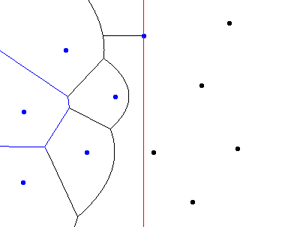
\includegraphics[scale=0.6]{images/fortune.png}
	\caption{Still frame from the Fortune's Algorithm animated gif \cite{fortunewiki}}\label{fig:fortune}
\end{figure}
\section{Graph structures}
\subsection{Voronoi Diagrams}
Voronoi diagrams are a way to partition space. Given a "random" sample of points an algorithm will create cells containing all points that are closer to the cell's seed point than all other seed points. 
\begin{figure}[h!]
	\centering
		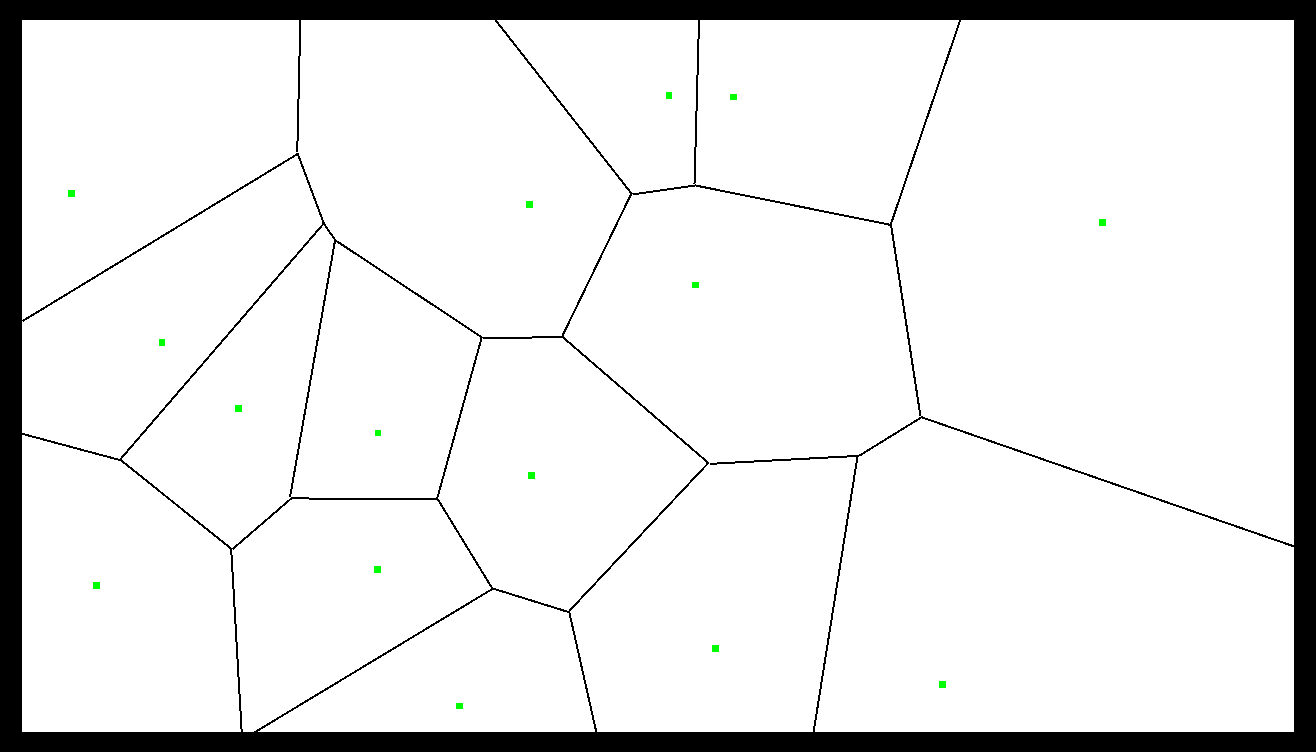
\includegraphics[scale=.2]{images/voronoi-unrelaxed}
		\caption{Voronoi diagram with 15 nodes.}
	\label{fig:pccs:voronoi}
\end{figure}
In figure~\ref{fig:pccs:voronoi} you see an example of a Voronoi diagram. The small dots in the cells are the sample points from which the cells were defined. With the irregular shapes that this gives us, we need to do some other steps before we get a workable partitioning. There are a few ways to 'unify' the shapes generated, we opted for Lloyd' algorithm, also known as Voronoi iteration or - relaxation. This algorithm calculates the centres of all the cells and uses these as new sample points for a new diagram. In figure~\ref{fig:lloydal} there is a visualization of this process.

\begin{figure}[h!]
\centering
\begin{subfigure}[b]{0.2\textwidth}
	\centering
	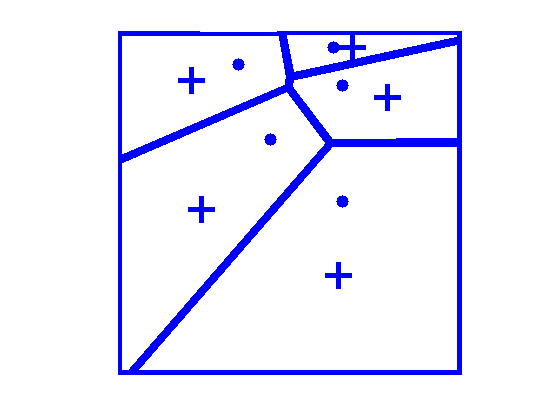
\includegraphics[width=\textwidth]{images/LloydsMethodIteration1.png}
	\caption{Lloyd's algorithm first iteration}
	\label{fig:lloyd1}
\end{subfigure}
~
\begin{subfigure}[b]{0.2\textwidth}
	\centering
	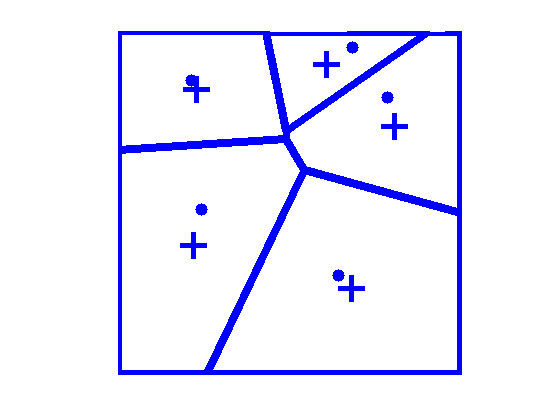
\includegraphics[width=\textwidth]{images/LloydsMethodIteration2.png}
	\caption{Lloyd's algorithm second iteration}
	\label{fig:lloyd2}
\end{subfigure}
~
\begin{subfigure}[b]{0.2\textwidth}
	\centering
	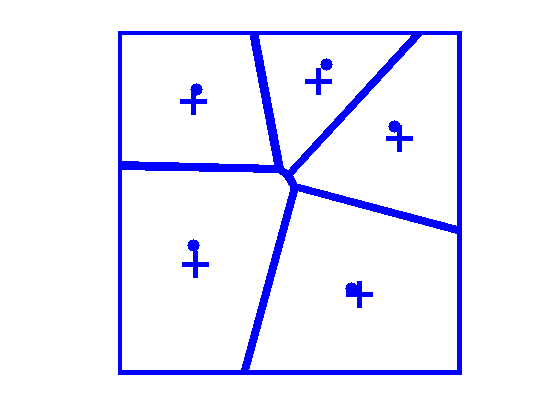
\includegraphics[width=\textwidth]{images/LloydsMethodIteration3.png}
	\caption{Lloyd's algorithm third iteration}
	\label{fig:lloyd3}
\end{subfigure}
~
\begin{subfigure}[b]{0.2\textwidth}
	\centering
		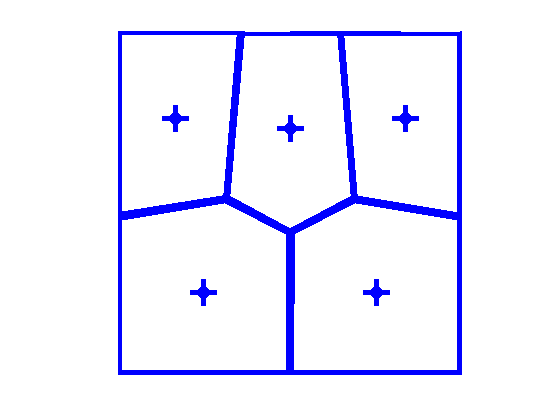
\includegraphics[width=\textwidth]{images/LloydsMethodIteration15.png}
		\caption{Lloyd's algorithm fifteenth iteration}
	\label{fig:lloyd15}
\end{subfigure}
\caption{Lloyd's algorithm \cite{lloydwiki}} \label{fig:lloydal}
\end{figure}
\subsection{Delaunay Triangulation}
The relation to the different Voronoi cells can be visually represented using a Delaunay triangulation. This results in an undirected graph which specifies neighbouring cells. In spatial partitioning this is of particular note, for with this information we can start to direct a path from one cell to another at any point in the entire game world. Thus, for example, being able to make certain cells inaccessible from specified directions, or make path-finding easier. Figure~\ref{fig:voronoidelaunay} shows a Voronoi tessellation with the relation of cells represented in a Delaunay triangulation. 
\begin{figure}[b]{}
\centering
	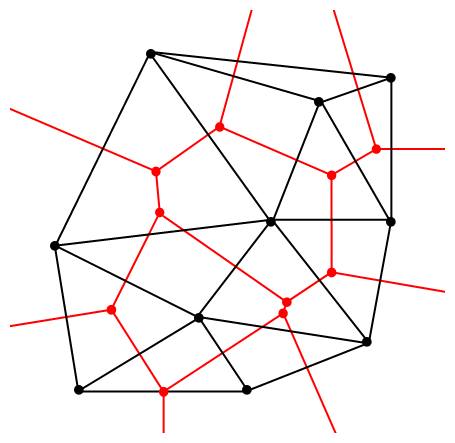
\includegraphics[scale=0.25]{images/Delaunay_Voronoi}
	\caption{Voronoi diagram with a Delaunay triangulation overlay \cite{delaunaywiki}} 
\label{fig:voronoidelaunay}
\end{figure}
The red and black lines represent the Voronoi and Delaunay edges respectively. With the red dots being the corners for the Voronoi cells and the black dots the nodes for the Delaunay triangulation {(as well as the seed nodes for the tessellation)}
\subsection{Connecting Graphs} \label{sec:connectinggraphs}
In the computational representation of these we use three object types: \emph{Centre, Corner and Edge}. The centre being the node of a Delaunay triangulation or the seed point of a Voronoi cell. Corners are exactly that, the corners of a Voronoi cell. These two have references to each other and others of their type that they are connected to. They are further connected by the final type; the edges. An edge is nothing more than a connection of corner to corner and centre to centre that convey both the Voronoi and Delaunay relation as shown in figure~\ref{fig:relation}.
\begin{figure}[h]
	\centering
	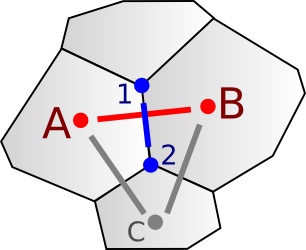
\includegraphics[scale=0.75]{images/edge-duality.png}
	\caption{The relational graph\cite{patel}}\label{fig:relation}
\end{figure}
The \emph{A,B} and \emph{1,2} represent the centres and corners respectively, with the lines representing their edges. The edge object holds a reference to these two groups of two nodes. 
\section{Defining a game world}
I did not want to use the diagram purely for the generation of landscapes or game-worlds. I wanted to define certain 'mission-spaces' in which players completes objectives and traverses to the next mission space where he/she finds one or more other players. This continues until all players have gathered in the last mission space. To create organic worlds, as well as the mission space in a more organic way I needed to nest two Voronoi diagrams.
\begin{figure}[ht]
	\centering
	\begin{subfigure}[b]{0.5\textwidth}
		\centering
		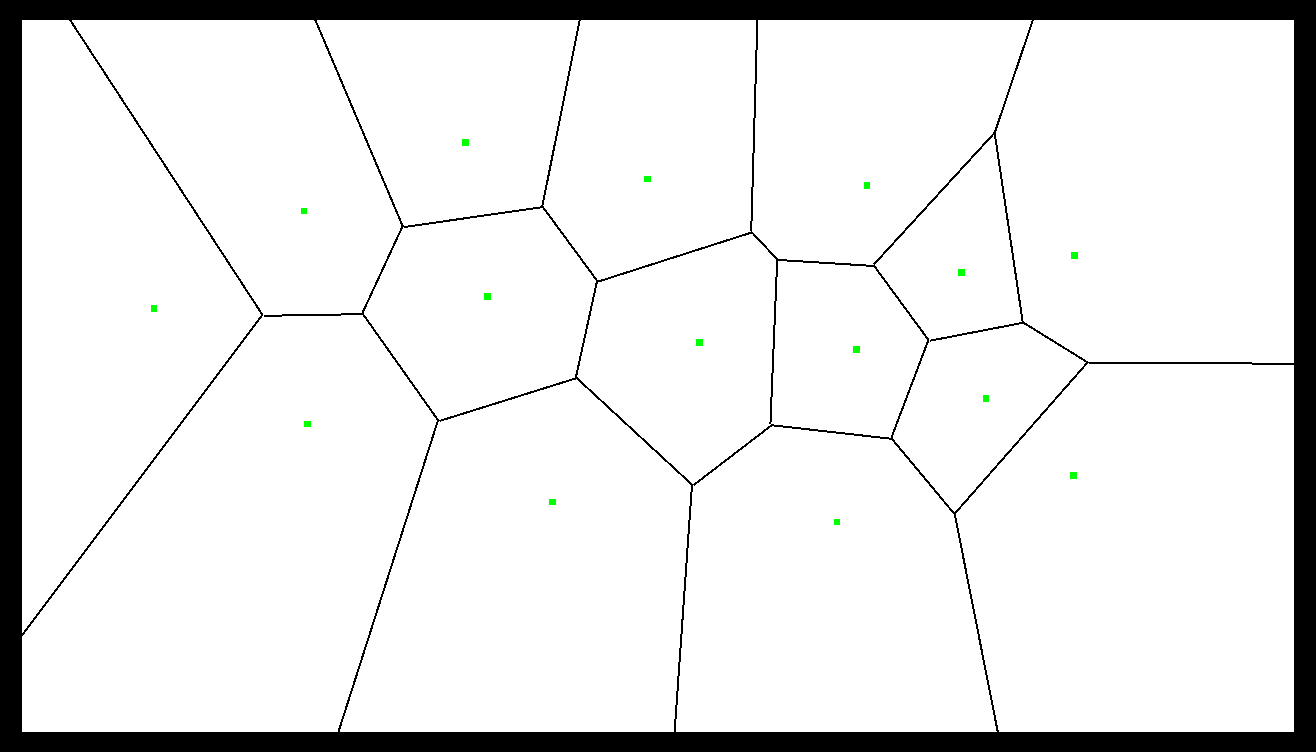
\includegraphics[width=\textwidth]{images/voronoipccs.png}
		\caption{Voronoi diagram}\label{fig:pccs:voronoiRelaxed}
	\end{subfigure}		
	~
	\begin{subfigure}[b]{0.5\textwidth}
		\centering
		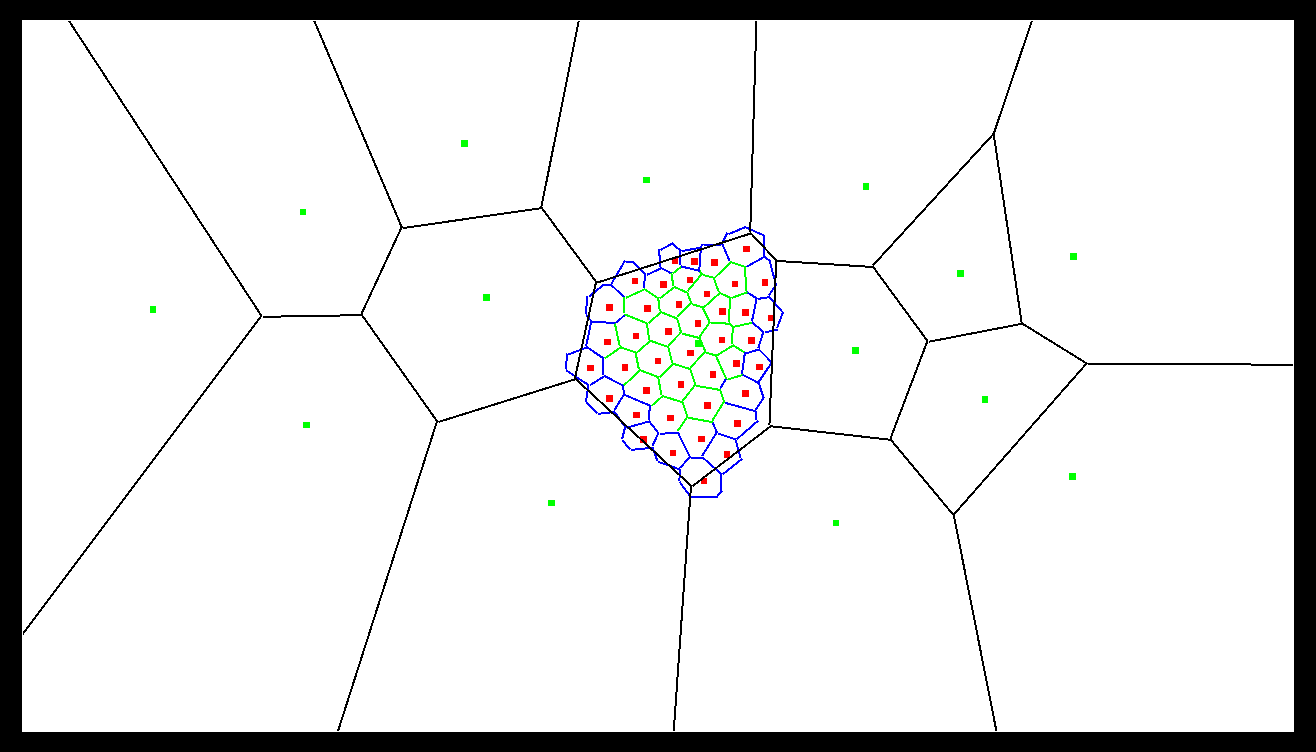
\includegraphics[width=\textwidth]{images/voronoi2pccs.png}
		\caption{Voronoi cell with children} \label{fig:pccs:voronoiNested}
	\end{subfigure}		
	\caption{ }\label{fig:vvn}
\end{figure}
In figure~\ref{fig:pccs:voronoiRelaxed} you see the generated world space. Each cell is one of the aforementioned mission spaces. These mission spaces get partitioned in another Voronoi diagram as seen in figure~\ref{fig:pccs:voronoiNested}. The outer cells are used to define borders between each other outer cell, whereas the inner cells define such things as objective location, terrain and vegetation.
\subsection{Nesting Voronoi diagrams}
There are several methods to nest these diagrams. The most obvious would be adding some random seed points within the outer cells and running the algorithm within the cell's bounds, but this has some drawbacks. As mentioned before, we used a sweep-line algorithm made by Steven Fortune~\cite{fortuneacm}. This algorithm is optimized for rectangular planes as the sweep-line itself is fixed and following the bounds of a polygon requires quite a bit of calculation. 

We opted for a simpler method that did not require any modification to the algorithms and techniques we were already using. This method uses the same plane as the outer cells and adds more seed points to this plane. After the algorithm did its job, we assign inner cells to outer cells by their very Voronoi property, distance to seed point. 
In figure~\ref{fig:pccs:voronoiwchild} you see the outer cells in red and the inner in black (with green seed points).
\begin{figure}[ht]
	\centering
	\begin{subfigure}[b]{0.5\textwidth}
	\centering
	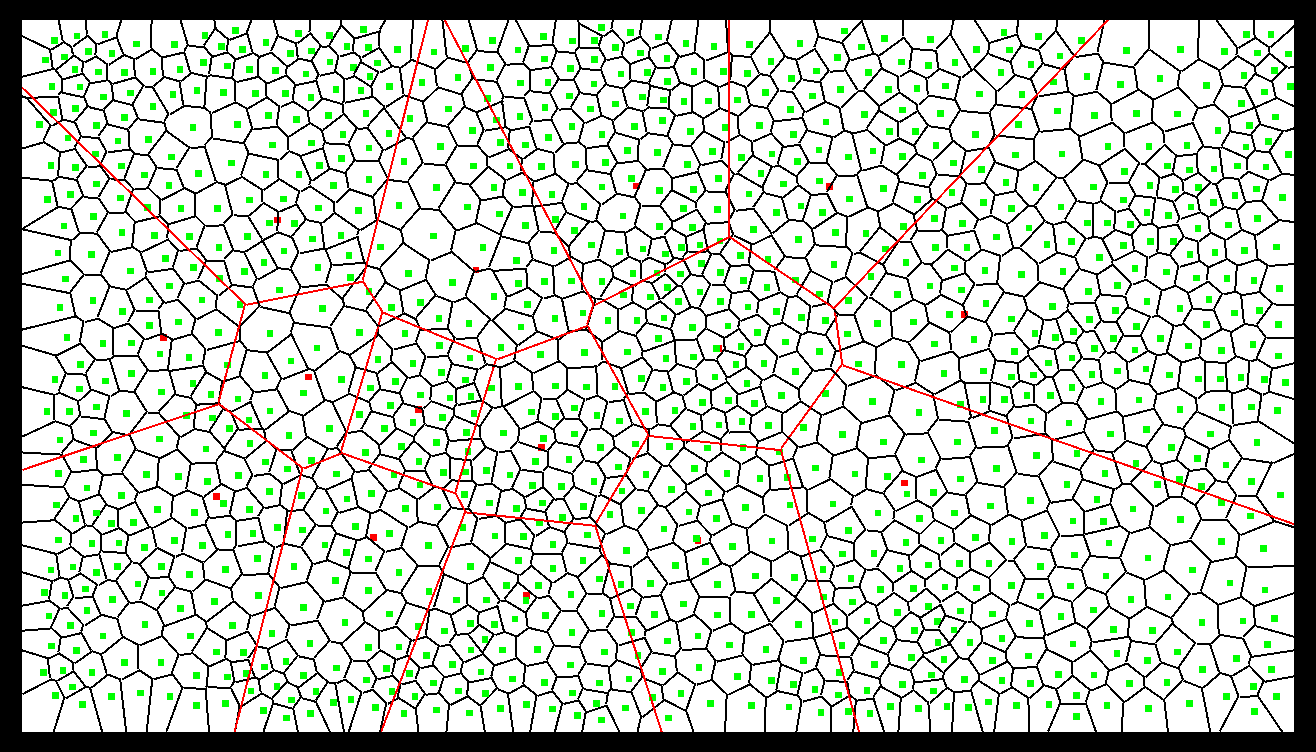
\includegraphics[width=\textwidth]{images/voronoiwchild.png}
	\caption{Voronoi diagram with inner and outer cells} \label{fig:pccs:voronoiwchild}
	\end{subfigure}
	~
	\begin{subfigure}[b]{0.5\textwidth}
	\centering
	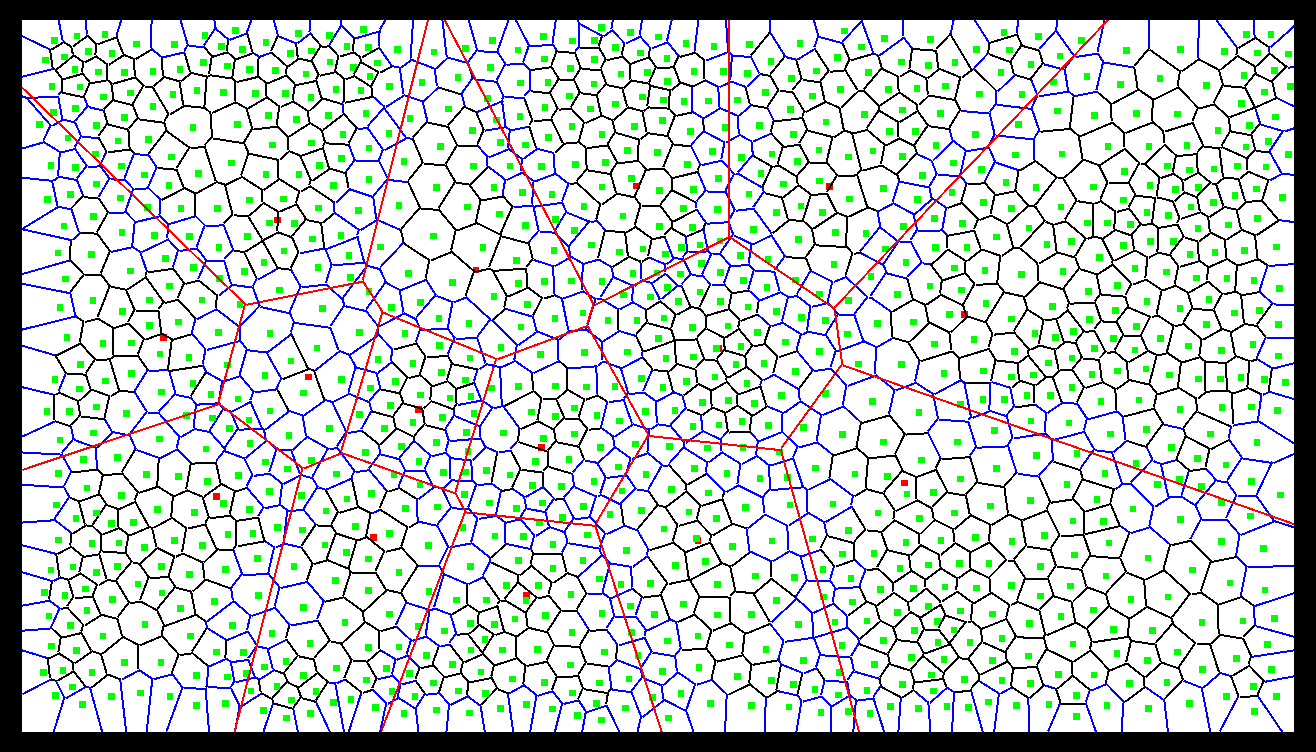
\includegraphics[width=\textwidth]{images/voronoiwchildborder.png}
	\caption{Voronoi diagram with inner and outer cells showing the border cells} \label{fig:pccs:voronoiwchildborders}
	\end{subfigure}
	\caption{ }\label{fig:children}
\end{figure}
In figure~\ref{fig:pccs:voronoiwchildborders} and \ref{fig:pccs:voronoiNested} you can see the results of the assignment. The blue cells indicate that they are on the border of their respective parent cell, 
\section{Finding possible paths}
In our game we wanted different players to start in their own mission spaces and gradually team up after overcoming a challenge in a mission space. For this I decided on a binary structure as shown in figure~\ref{fig:bintree}. All nodes in this tree represent a mission space, where the leaf nodes represent the player's starting mission space. For this example I used eight players that team up after every mission. Thus player 1 teams up with 2 (team A) and 3 with 4 (team B) after that team A and B get together for the third node. 
\begin{figure}[h]
	\centering
	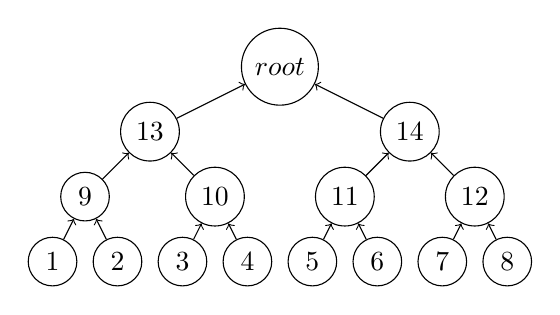
\begin{tikzpicture}[scale=0.55]
		\node[circle,draw](z){$root$} [<-]
			child [sibling distance=6cm] {node[circle,draw](a){13}
				child [sibling distance=3cm]{node[circle,draw](b){9}
					child [sibling distance=1.5cm] {node[circle,draw](c){1}}
					child [sibling distance=1.5cm] {node[circle,draw](d){2}}
				}
				child [sibling distance=3cm] {node[circle,draw](e){10}
					child [sibling distance=1.5cm] {node[circle,draw](f){3}}
					child [sibling distance=1.5cm] {node[circle,draw](g){4}}
				}
			}
			child [sibling distance=6cm] {node[circle,draw](h){14}
				child [sibling distance=3cm] {node[circle,draw](i){11}
					child [sibling distance=1.5cm] {node[circle,draw](j){5}}
					child [sibling distance=1.5cm] {node[circle,draw](k){6}}
				}
				child [sibling distance=3cm] {node[circle,draw](l){12}
					child [sibling distance=1.5cm] {node[circle,draw](m){7}}
					child [sibling distance=1.5cm] {node[circle,draw](n){8}}
				}
			};
			
	\end{tikzpicture}	
	\caption{Binary tree where each node represents a mission space. The leaves represent the starting position of players.} \label{fig:bintree}
\end{figure}
To realize this structure we needed to find this tree (or similar, depending on the number of players) in the Delaunay graph of the mission spaces. This is a recursive brute force method that searches all possible paths for one that fits the description. See figure~\ref{fig:ludo:delaunays} for a good example of the outcome.

Due to the structures we used the Delaunay edges are interchangeable for the Voronoi edges. Running the brute force algorithm in figure~\ref{fig:ludo:voronoi} results in figure~\ref{fig:ludo:voronoiopen}. 
\begin{figure}[h]
	\begin{subfigure}[b]{0.5\textwidth}
		\centering
		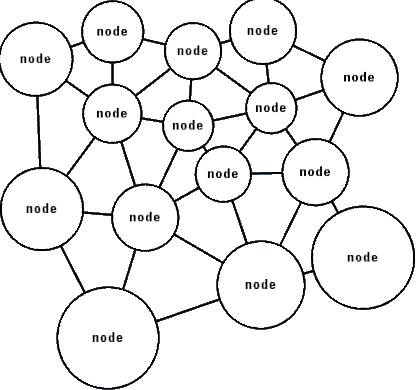
\includegraphics[width=0.4\textwidth]{images/ludodelaunay.png}
		\caption{Delaunay triangulation. (made with Ludoscope)}\label{fig:ludo:delaunay}
	\end{subfigure}
	
	\begin{subfigure}[b]{0.5\textwidth}
		\centering
		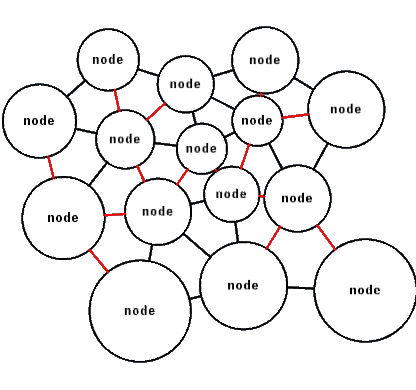
\includegraphics[width=0.4\textwidth]{images/ludodelaunaypaths.png}
		\caption{Delaunay triangulation where the red edges are the edges of figure~\ref{fig:bintree} that was found in this graph. (made with Ludoscope)}\label{fig:ludo:delaunaypaths}
	\end{subfigure}
	\caption{ }\label{fig:ludo:delaunays}
\end{figure}
\begin{figure}[h]
	\centering
	\begin{subfigure}[b]{0.5\textwidth}
		\centering
		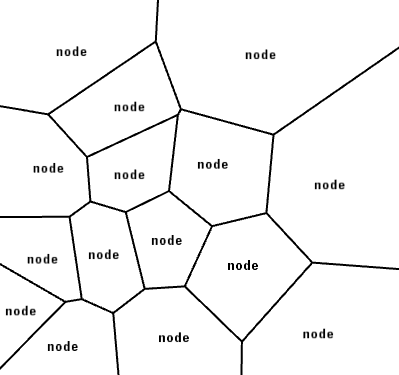
\includegraphics[width=0.4\textwidth]{images/ludovoronoi.png}
		\caption{Voronoi diagram. (made with Ludoscope)}\label{fig:ludo:voronoi}
	\end{subfigure}
	
	\begin{subfigure}[b]{0.5\textwidth}
		\centering
		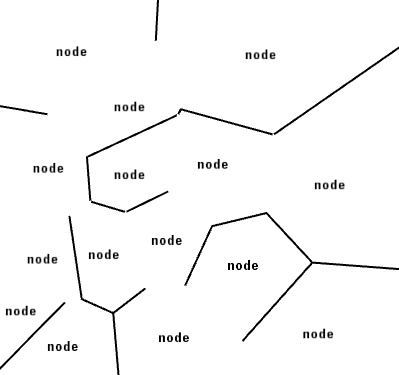
\includegraphics[width=0.4\textwidth]{images/ludovoronoiopen.png}
		\caption{Voronoi diagram where the black lines represent physical borders, forcing the players to travel to the next space as dictated by the algorithm. (made with Ludoscope)}\label{fig:ludo:voronoiopen}
	\end{subfigure}
	\caption{ }\label{fig:ludo:voronois}
\end{figure}
\section{Conclusion}
A single Voronoi diagram is a powerful tool for spatial partitioning and can create some amazing organic shapes. However, when the devil is in the details, just merely generating a lot of Voronoi cells make a world cluttered an disorganized. it can even give technical limitations with two, or more, seed points being to close to one and other. To solve this problem I tried to nest two diagrams in each other, creating a top and bottom layer.
With these two structures put in place. We can define, not only the entire world with a organic feel, but give the different top layer cells different attributes such as its own climate. Creating a feel for depth and complexity that a single Voronoi diagram might lack.
\newpage
\begin{thebibliography}{0}

\bibitem{patel}
	Amit Patel,\newline
	\emph{Polygonal Map Generation for Games},\newline
	Stanford University,\newline
	\url{http://www-cs-students.stanford.edu/~amitp/game-programming/polygon-map-generation}

\bibitem{lloydwiki}
	Wikipedia Community,\newline
	\emph{Lloyd's Algorithm},\newline
	\url{http://en.wikipedia.org/wiki/Lloyd's_algorithm}

\bibitem{delaunaywiki}
	Wikipedia Community,\newline
	\emph{Delaunay Triangulation}, \newline
	\url{http://en.wikipedia.org/wiki/Delaunay_triangulation}

\bibitem{fortuneacm}
	Steven Fortune,\newline
	\emph{A sweepline} [sic] \emph{algorithm for Voronoi Diagrams}, \newline
	1986. ISBN 0-89791-194-6
\bibitem{sullivancpp}
	Shane O'Sullivan,\newline
	\emph{VoronoiDiagramGenerator},\newline
	(Fortune's algorithm in C++)
	\url{http://mapviewer.skynet.ie/voronoi.html}
\bibitem{fortunewiki}
	Wikipedia Community,\newline
	\emph{Fortune's Algorithm}
	\url{http://en.wikipedia.org/wiki/Fortune's_algorithm}
\end{thebibliography}

\end{document}
